\section{Metodologia}
A pré configuração estabelecida para a modulação e demodulação FM consiste no $K_{f} =$ 100 até 10.000 à passos de 100, criação das variáveis $samp_{rate} = 200.000$, $f_{m} = 1.000$, $f_{c} = 10.000$ e $f_{deri} = 10.000$, conforme Figura \ref{fig:pre_config}.

\begin{figure}[!htb]
    \centering
    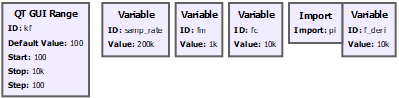
\includegraphics[scale=0.7]{Imagens/pre configuracao.PNG}
    \caption{Criação e configuração das variáveis.}
    \label{fig:pre_config}
\end{figure}


\subsection{Modulador FM}
Na modulação FM, foi criado um sinal cosseno de amplitude 1 e frequência $f_{m}$ através do bloco \textit{signal source}, passando pelo bloco \textit{Moving Average} no qual é utilizado para calcular a média móvel do sinal de entrada, facilitando a detecção de tendências ou a redução de ruído.
Sua escala foi calculada através da equação \ref{eq:moving_average}.

\begin{equation}
   Scale =  \frac{samp_{rate}}{2 \cdot f_{m} \cdot 1024}
   \label{eq:moving_average}
\end{equation}

Após isso, o sinal é multiplicado pela constante $K_{f}$, adicionado a constante $f_{c}$, passando pelo bloco \textit{Throttle} ajustando o processamento do computador para a simulação. E por fim, utilizando o bloco VCO \textit{(Voltage Controlled Oscillator)} para controlar a amplitude da onda através da amplitude do sinal de entrada, com uma sensibilidade de $2\pi$, conforme Figura \ref{fig:modulacao}.

\begin{figure}[!htb]
    \centering
    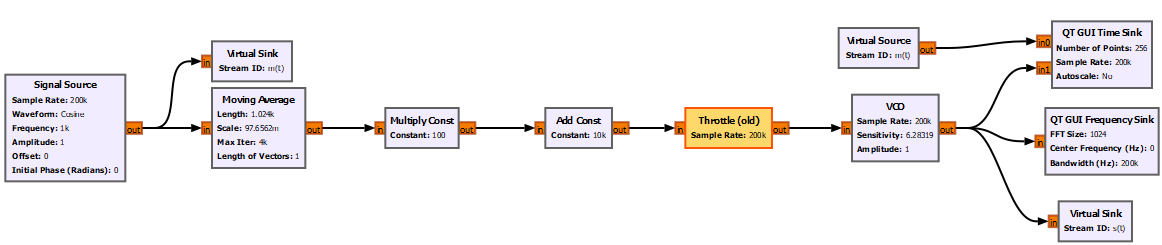
\includegraphics[width=0.5\textwidth]{Imagens/Modulacao_FM.PNG}
    \caption{Sinal modulado em frequência.}
    \label{fig:modulacao}
\end{figure}

\subsection{Demodulador FM}


A demodulação de um sinal FM se inicia com o passo descrito pela Equação \ref{eq09}, onde a mensagem é obtida através da derivação do sinal recebido. Dessa forma, a mensagem é replicada para a amplitude do sinal. Esse processo é uma transformação do sinal FM em AM. Esse processo foi implementado no \textit{GNU Radio} conforme Figura \ref{fig:dem_01}.

O bloco \textit{High Pass Filter}, que realiza a função de um filtro passa-altas, foi escolhido para performar a limitação da banda explicitada na Figura \ref{fig01}. Dessa forma, para uma conversão bem sucedida, deve-se escolher parâmetros como frequência de corte e largura de transição adequadamente. A frequência de corte influenciará na banda que será rejeitada e qual banda será passada. Assim, escolheu-se uma frequência de corte de $10 kHz$, devido à frequência da mensagem modulada. Além disso, a largura de transição foi de $100 Hz$, para que o filtro performe bem na atenuação. 

\begin{figure}[!htb]
    \centering
    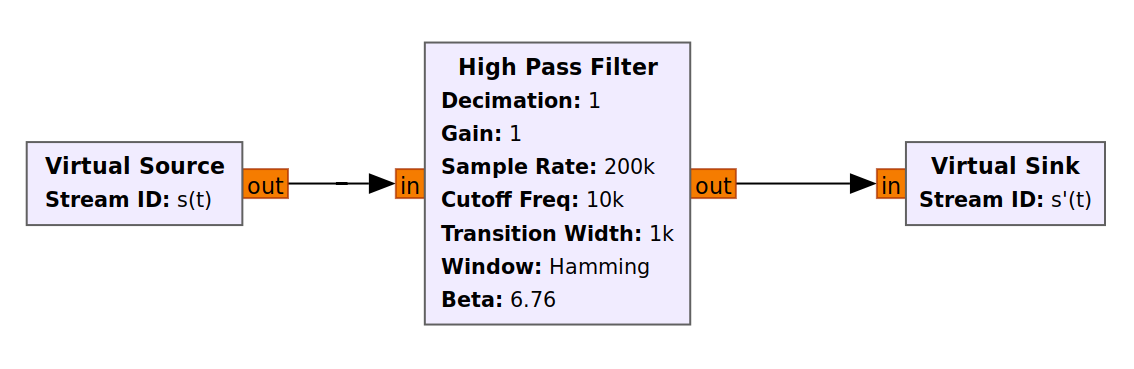
\includegraphics[width=1\linewidth]{Imagens/dem_01.png}
    \caption{derivação do sinal FM}
    \label{fig:dem_01}
\end{figure}

Uma vez que a conversão foi realizada, utiliza-se as técnicas de demodulação de um sinal AM. Neste caso, multiplica-se o sinal por ele mesmo, a fim de que o sinal volte à banda base. Essa operação é realizada utilizando o bloco \textit{Multiply}. Posteriormente, é realizada uma filtragem da banda base, com o bloco \textit{Low Pass Filter}. Assim, novamente os parâmetros de um filtro devem ser escolhidos de forma adequada. A frequência de corte deve ser aquela próxima à frequência da mensagem e a largura de transição deve ser escolhida de forma que bandas ou componentes adjacentes sejam excluídas. Assim, a frequência de corte foi $1 kHz$ e a banda de transição $100 Hz$. Esse bloco de operação pode ser visualizado na Figura \ref{demod_02}.

\begin{figure}[!htb]
    \centering
    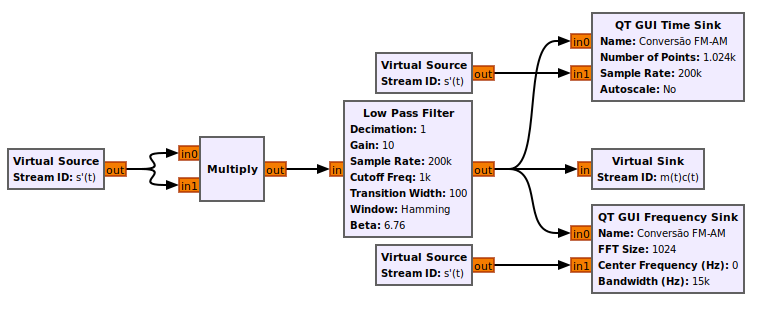
\includegraphics[width=1\linewidth]{Imagens/fig:dem_02.png}
    \caption{demodulação AM}
    \label{demod_02}
\end{figure}

Da mesma forma como ocorre com demodulações AM convencionais, deve-se rejeitar a influência da portadora antes de realizar a transformada inversa de \textit{Fourier} para que o sinal volte ao domínio do tempo, e a mensagem possa ser interpretada. Assim, utiliza-se uma conversão do sinal para o domínio complexo, remove-se a componente DC, $f = 0Hz$, e se converte o sinal para o domínio real. Após esse processo, obtém-se o sinal estimado. Essas operações podem ser vistas na Figura \ref{fig03}.

\begin{figure}[!htb]
    \centering
    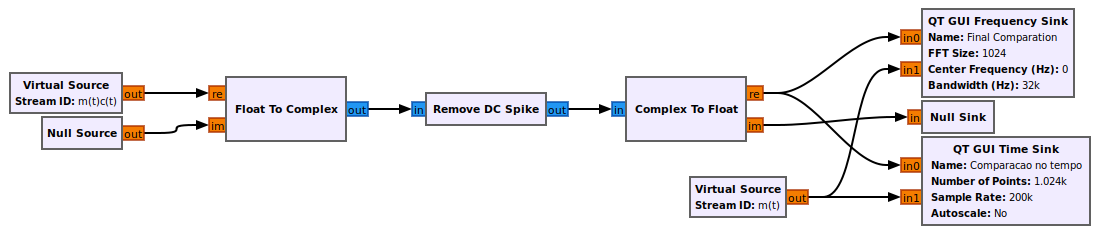
\includegraphics[width=1\linewidth]{Imagens/fig:dem_03.png}
    \caption{remoção de nível DC}
    \label{fig03}
\end{figure}